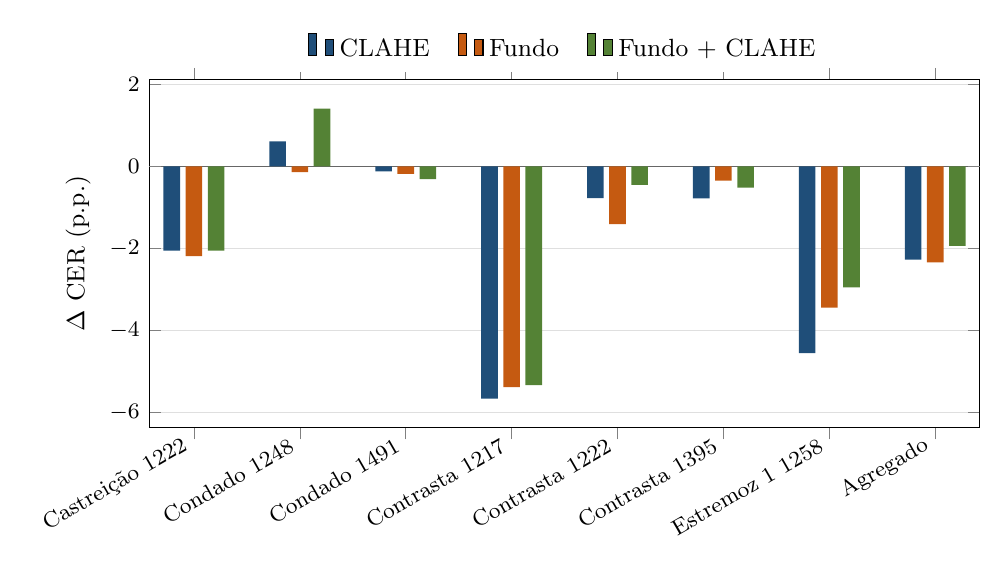
\begin{tikzpicture}
\begin{axis}[
  ybar,
  bar width=6pt,
  width=\linewidth,
  height=6cm,
  xtick={0,...,7},
  xticklabels={{Castreição 1222},{Condado 1248},{Condado 1491},{Contrasta 1217},{Contrasta 1222},{Contrasta 1395},{Estremoz 1 1258},{Agregado}},
  ylabel={$\Delta$ CER (p.p.)},
  /pgf/number format/use comma,
  /pgf/number format/precision=1,
  /pgf/number format/fixed,
  ymajorgrids,
  grid style={gray!25},
  enlarge x limits=0.06,
  tick label style={font=\footnotesize},
  label style={font=\small},
  x tick label style={rotate=30, anchor=east},
  extra y ticks={0}, extra y tick labels={}, extra y tick style={grid=major, grid style={black!60}},
  legend style={at={(0.5,1.02)}, anchor=south, legend columns=-1, draw=none, font=\small, /tikz/every even column/.append style={column sep=8pt}}
]
\addplot[fill={rgb,255:red,31;green,78;blue,121}, draw=none] coordinates {(0,-2.0572) (1,0.6089) (2,-0.1247) (3,-5.6604) (4,-0.7731) (5,-0.7799) (6,-4.5510) (7,-2.2747)};
\addplot[fill={rgb,255:red,197;green,90;blue,17}, draw=none] coordinates {(0,-2.1858) (1,-0.1405) (2,-0.1870) (3,-5.3836) (4,-1.4097) (5,-0.3466) (6,-3.4440) (7,-2.3414)};
\addplot[fill={rgb,255:red,84;green,130;blue,53}, draw=none] coordinates {(0,-2.0572) (1,1.4052) (2,-0.3117) (3,-5.3333) (4,-0.4548) (5,-0.5199) (6,-2.9520) (7,-1.9412)};
\legend{CLAHE,Fundo,Fundo + CLAHE}
\end{axis}
\end{tikzpicture}
